\section{Sequential Experimentation}
\label{sequential}
\indent

Regarding the prior described lemas, we shall now assess wether if the linear algebra approach presents performance improvements when compared with the relational one. 
Before we discuss the measured performance results in the following section, we will briefly summarise characteristics of the multicore platform in our test suite, and present an overview of the performed tunings.\\

Throughout all experiments, the same platform was used. The system, referenced as compute node 652-1, has two Intel\textsuperscript{\textregistered} Xeon\textsuperscript{\textregistered} E5-2670v2 (Ivy Bridge architecture) sharing 64 GB of DDR3 RAM, 1333 MHz, accessed through 4 memory channels. Table \ref{table:characterization} fully characterises the hardware features of the test platform:

\begin{table}[H]
\centering
  \begin{tabular}{ | L{3.5cm} | R{5cm} | }
  
    \hline
    System & compute-652-1 \\ \hline \hline
        \# CPUs & 2\\ \hline
    CPU & Intel\textsuperscript{\textregistered} Xeon\textsuperscript{\textregistered} E5-2670v2\\ \hline 
    Architecture & Ivy Bridge \\ \hline 
    \# Cores per CPU & 10 \\ \hline 
    \# Threads per CPU & 20\\ \hline 
    Clock Freq. & 2.5 GHz\\ \hline \hline 
    L1 Cache & 320KB \newline 32KB per core\\ \hline 
    L2 Cache & 2560KB  \newline  256KB per core \newline\\ \hline 
    L3 Cache & 25600KB \newline shared \\ \hline \hline 
    Inst. Set Ext. & SSE4.2 \& AVX \\ \hline 
        \#Memory Channels & 4\\ \hline \hline

    Vendors Announced Peak Memory BW & 59.7 GB/s\\ \hline
    Measured\footnote{Stream Benchamrk} Peak Memory BW & 58.5GB/s\\ \hline
  \end{tabular}
     \caption{Architectural characteristics of the evaluation platform.}
     \label{table:characterization}
\end{table}

The software used for both relational and linear algebra, and the corresponding versions are stated bellow:

\begin{itemize}
\item Linear Algebra: 
    \begin{itemize}
    \item Compiler: ICC version 16.0.0 (GCC version 4.4.6 compatibility)
    \begin{itemize}
        \item no vectorization: -O3 -std=c99 -no-vec -farray-notation 
        \item vectorization: -O3 -std=c99 -farray-notation -xAVX -vec-report7
    \end{itemize}
    \item Intel\textsuperscript{\textregistered} MKL Version	11.3
    \begin{itemize}
        \item Link line: -lmkl\_intel\_lp64 -lmkl\_core -lmkl\_sequential -lpthread -lm
    \end{itemize}
        \end{itemize}

\vspace{0.35cm}
    \item Relational Algebra (PostgreSQL version 9.6+);
    \begin{itemize}
        \item Built with the following dependencies:
        \begin{itemize}
            \item GCC version 4.9.0
            \item Python 2.6.6
        \end{itemize}
           \end{itemize}
\end{itemize}

PostgreSQL was compiled specifically for the test platform, to fully take advantage of the available computing resources. 

\subsection{Tuning the relational algebra engine}
Database, application, and storage servers ship with a large number of configuration parameters like buffer cache sizes, number of I/O daemons, and parameters input to the database query optimiser. Finding good settings for these parameters is a challenging task because of the complex ways in which parameter settings can affect performance. The parameters shared\_buffers, effective\_cache\_size, and work\_mem, were adjusted accordingly, with  shared\_buffers begin set to 2GB, effective\_cache\_size being set to 64GB, and work\_mem being set to 25MB. In order to further speed up RA queries, indexes were created for all the database tables.


\subsection{Tuning sparse CSC and CSR methods to assist data level parallelism}

Efficient SSE vectorisation was achieved  in both versions of the linear algebra approach. The usage of the performant Intel Math Kernel Library (MKL) fully assisted vectorisation of the dot product between sparse matrices and sparse matrix vector, on the CSR version.\par 
The compiler was also instructed via auto vectorisation hints, and user mandated vectorisation. The non existence of vector dependencies, when verified, was also explicitly included.\par 
Alignment of data and data structures can affect performance. 
In the memory allocation alignment all data was aligned  according to cache line size. Regarding the access alignment,
for AVX, alignment to 32-byte boundaries (8 SP chunks) allowed a single reference to a cache line to move 8-SP numbers into the registers. 
The compiler was instructed to to assume that all CSC and CSR arrays are aligned on an 32-byte boundary.

\subsection{Tuning RA and LA approaches}


We conducted experiments on the simplified TPC-H  query-1, shown in listing \ref{used_query_1}, similar to the one presented in listing \ref{query_1}. 
The experiments focused a variety of datasets ranging from 1GB to 32GB. An overview of their characteristics appears in table \ref{table:dataset_info}. 

The CSC format requires a  larger  overall space for data, but it allowed us to simplify several algorithms and improve the overall perfomance.

\lstinputlisting[caption=SQL code for the simplified TPC-H query 1 used on the experimentation, label=used_query_1]{sql/used_query_1.sql} %input de um ficheiro





\end{multicols}

\noindent

\begin{table}[H]
\centering
  \footnotesize
     \caption{Overview of the produced sparse matrices used in evaluation study.}
  \begin{tabular}{ | L{0.75cm} | L{3.25cm} | L{3.25cm} | L{3.25cm} | L{3.25cm} | L{1.1cm} | L{1.1cm} | }
  
    \hline
    
  \multirow{2}{*}{Dataset} 	&	Measure Matrix Quantity			&	Projection Matrix return flag			&	Projection Matrix line status			&	Projection Matrix ship date			&	\multicolumn{2}{| L{2.4cm} |}{Overall SP Space Required}			  \\ \cline{2-7}

	&	Dimensions, Nonzeros, CSR space, CSC space			&	Dimensions, Nonzeros, CSR space, CSC space			&	Dimensions, Nonzeros, CSR space, CSC space			&	Dimensions, Nonzeros, CSR space, CSC space			&	CSR format	&	CSC format	  \\ \hline
1	& (	6001215	$\times$	6001215	) & (	3	$\times$	6001215	) & (	5	$\times$	6001215	) & (	2531	$\times$	6001215	) &		&		  \\ \cline{2-5}
	&	nnz:		6001215	&	nnz:		6001215	&	nnz:		6001215	&	nnz:		6001215	&		&		  \\ \cline{2-5}
	& CSR:	69	 MB CSC: 	69	MB & CSR:	46	 MB CSC: 	69	MB & CSR:	46	 MB CSC: 	69	MB & CSR:	46	 MB CSC: 	69	MB &	206	MB &	275	MB  \\ \hline
2	& (	11997996	$\times$	11997996	) & (	3	$\times$	11997996	) & (	5	$\times$	11997996	) & (	2531	$\times$	11997996	) &		&		  \\ \cline{2-5}
	&	nnz:		11997996	&	nnz:		11997996	&	nnz:		11997996	&	nnz:		11997996	&		&		  \\ \cline{2-5}
	& CSR:	137	 MB CSC: 	137	MB & CSR:	92	 MB CSC: 	137	MB & CSR:	92	 MB CSC: 	137	MB & CSR:	92	 MB CSC: 	137	MB &	412	MB &	549	MB  \\ \hline
4	& (	23996604	$\times$	23996604	) & (	3	$\times$	23996604	) & (	5	$\times$	23996604	) & (	2531	$\times$	23996604	) &		&		  \\ \cline{2-5}
	&	nnz:		23996604	&	nnz:		23996604	&	nnz:		23996604	&	nnz:		23996604	&		&		  \\ \cline{2-5}
	& CSR:	275	 MB CSC: 	275	MB & CSR:	183	 MB CSC: 	275	MB & CSR:	183	 MB CSC: 	275	MB & CSR:	183	 MB CSC: 	275	MB &	824	MB &	1098	MB  \\ \hline
8	& (	47989007	$\times$	47989007	) & (	3	$\times$	47989007	) & (	5	$\times$	47989007	) & (	2531	$\times$	47989007	) &		&		  \\ \cline{2-5}
	&	nnz:		47989007	&	nnz:		47989007	&	nnz:		47989007	&	nnz:		47989007	&		&		  \\ \cline{2-5}
	& CSR:	549	 MB CSC: 	549	MB & CSR:	366	 MB CSC: 	549	MB & CSR:	366	 MB CSC: 	549	MB & CSR:	366	 MB CSC: 	549	MB &	1648	MB &	2197	MB  \\ \hline
16	& (	95988640	$\times$	95988640	) & (	3	$\times$	95988640	) & (	5	$\times$	95988640	) & (	2531	$\times$	95988640	) &		&		  \\ \cline{2-5}
	&	nnz:		95988640	&	nnz:		95988640	&	nnz:		95988640	&	nnz:		95988640	&		&		  \\ \cline{2-5}
	& CSR:	1099	 MB CSC: 	1099	MB & CSR:	732	 MB CSC: 	1099	MB & CSR:	732	 MB CSC: 	1099	MB & CSR:	732	 MB CSC: 	1099	MB &	3296	MB &	4394	MB  \\ \hline
32	& (	192000551	$\times$	192000551	) & (	3	$\times$	192000551	) & (	5	$\times$	192000551	) & (	2531	$\times$	192000551	) &		&		  \\ \cline{2-5}
	&	nnz:		192000551	&	nnz:		192000551	&	nnz:		192000551	&	nnz:		192000551	&		&		  \\ \cline{2-5}
	& CSR:	2197	 MB CSC: 	2197	MB & CSR:	1465	 MB CSC: 	2197	MB & CSR:	1465	 MB CSC: 	2197	MB & CSR:	1465	 MB CSC: 	2197	MB &	6592	MB &	8789	MB  \\ \hline
  \end{tabular}
     \label{table:dataset_info}
\end{table}
\newpage

\begin{multicols}{2}

\subsection{Experimental results analysis}

Figure \ref{fig:time_la_vs_ra} plots the measured execution for a range of datasets, and both linear and relational algebra approaches.

Denote that the presented values were selected through the K-Best technique, with K=3, from 50 samples. 

For the linear algebra approach we present the best solution from CSR and CSC format. The presented linear algebra solution in figure \ref{fig:time_la_vs_ra} is the one using CSR and format and  Intel MKL version 11.3. \par
The experiment presented in the current section focus on the best possible sequential solutions for both relational and linear algebra versions. The parallel PostgreSQL line was only introduced to elucidate the parallel  goal to achieve in the LA versions discussed in later sections of this report, and discuss future potential improvements of our linear algebra system. 

As shown, the coding effort to tune sparse CSR methods to assist data level parallelism revealed itself fruitful. However, a further analysis should be produced in order to fully potentiate vectorisation opportunities and optimisations.\par 

\begin{figure}[H]
\centering
\caption{Execution time for the  simplified query-1 from TPC-H benchmark, for different scale factors (dataset sizes from 1GB to 32GB).}
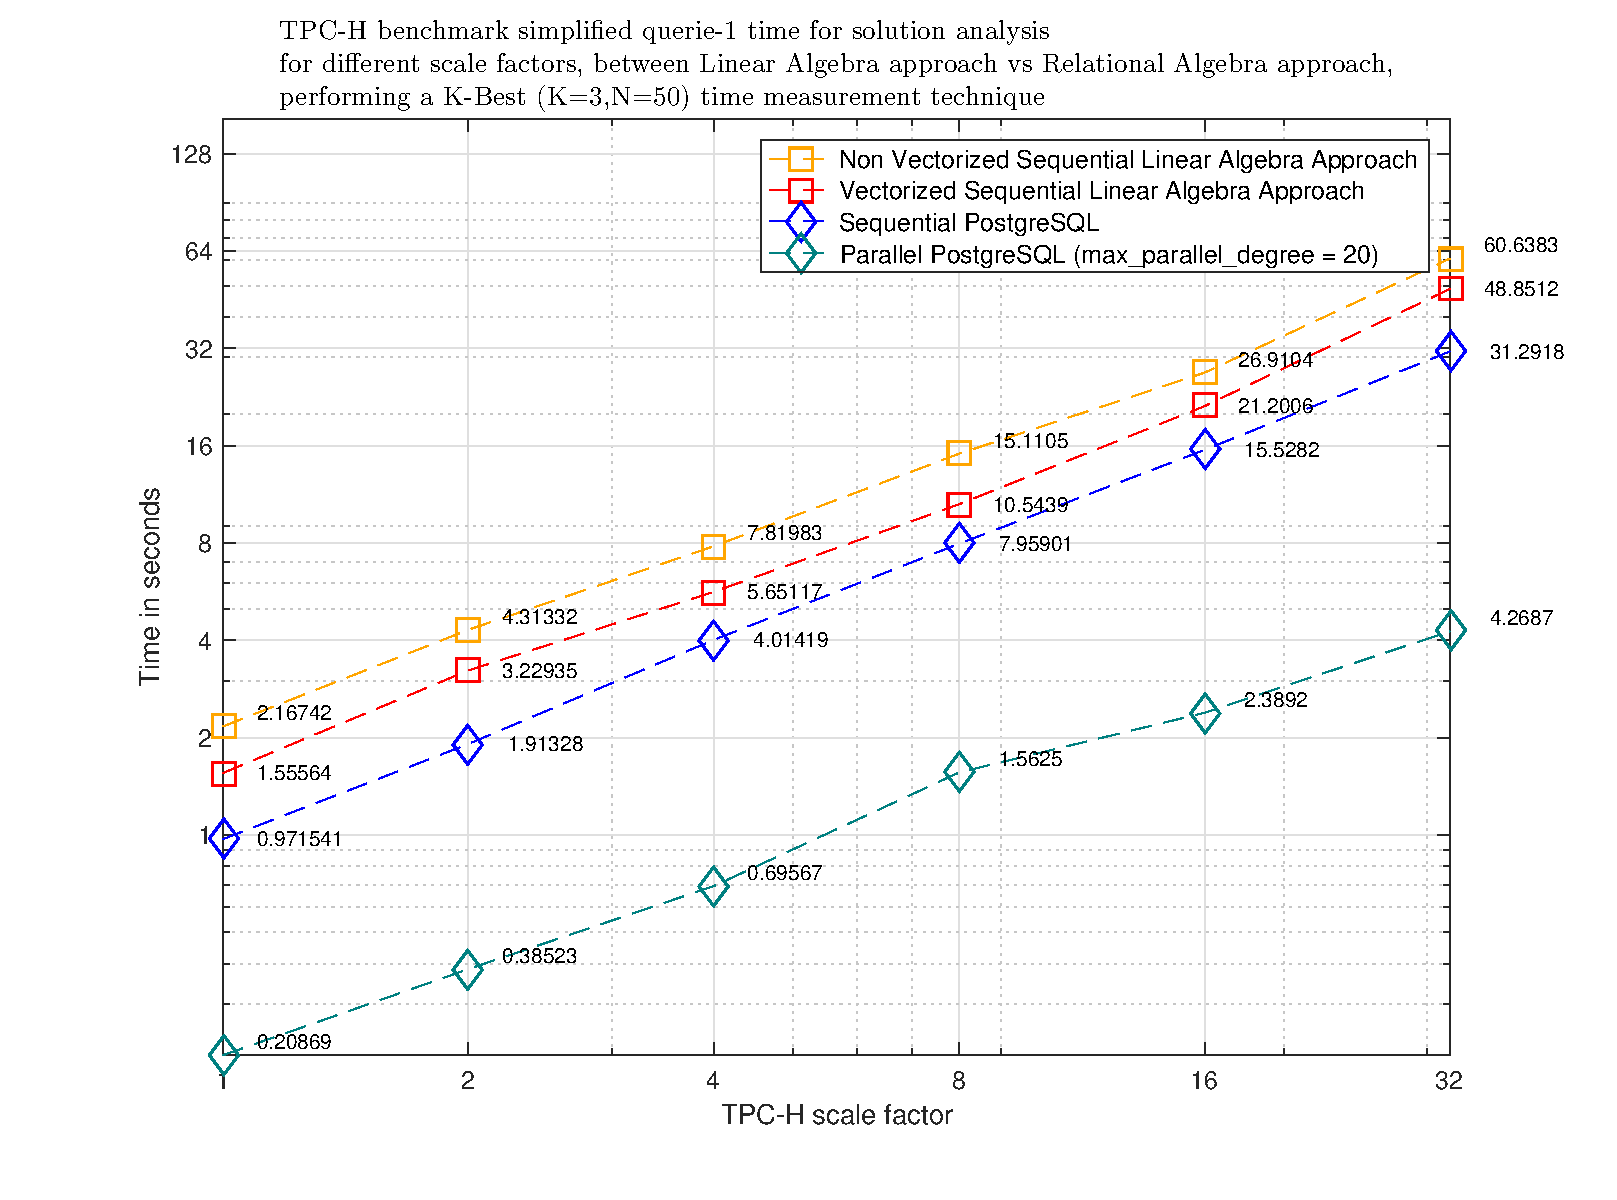
\includegraphics[width=1\columnwidth]{eps/TIME_LA_vs_RA_1st.eps}
\label{fig:time_la_vs_ra}
\end{figure}




